\documentclass[compress]{beamer}
\usepackage{ifthen,verbatim}

\newcommand{\isnote}{}
\xdefinecolor{lightyellow}{rgb}{1.,1.,0.25}
\xdefinecolor{darkblue}{rgb}{0.1,0.1,0.7}

%% Uncomment this to get annotations
%% \def\notes{\addtocounter{page}{-1}
%%            \renewcommand{\isnote}{*}
%% 	   \beamertemplateshadingbackground{lightyellow}{white}
%%            \begin{frame}
%%            \frametitle{Notes for the previous page (page \insertpagenumber)}
%%            \itemize}
%% \def\endnotes{\enditemize
%% 	      \end{frame}
%%               \beamertemplateshadingbackground{white}{white}
%%               \renewcommand{\isnote}{}}

%% Uncomment this to not get annotations
\def\notes{\comment}
\def\endnotes{\endcomment}

\setbeamertemplate{navigation symbols}{}
\setbeamertemplate{headline}{\mbox{ } \hfill
\begin{minipage}{5.5 cm}
\vspace{-0.75 cm} \small
\end{minipage} \hfill
\begin{minipage}{4.5 cm}
\vspace{-0.75 cm} \small
\begin{flushright}
\ifthenelse{\equal{\insertpagenumber}{1}}{}{Jim Pivarski \hspace{0.2 cm} \insertpagenumber\isnote/\pageref{numpages}}
\end{flushright}
\end{minipage}\mbox{\hspace{0.2 cm}}\includegraphics[height=1 cm]{../cmslogo} \hspace{0.1 cm} \includegraphics[height=1 cm]{../tamulogo} \hspace{0.01 cm} \vspace{-1.05 cm}}

\begin{document}
\begin{frame}
\vfill
\begin{center}
\textcolor{darkblue}{\Large Miscellaneous track-based alignment updates}

\vfill
\begin{columns}
\column{0.3\linewidth}
\begin{center}
\large
\textcolor{darkblue}{Jim Pivarski}
\end{center}
\end{columns}

\begin{columns}
\column{0.3\linewidth}
\begin{center}
\scriptsize
{\it Texas A\&M University}
\end{center}
\end{columns}

\vfill
25 September, 2009

\end{center}
\end{frame}

%% \begin{notes}
%% \item This is the annotated version of my talk.
%% \item If you want the version that I am presenting, download the one
%% labeled ``slides'' on Indico (or just ignore these yellow pages).
%% \item The annotated version is provided for extra detail and a written
%% record of comments that I intend to make orally.
%% \item Yellow notes refer to the content on the {\it previous} page.
%% \item All other slides are identical for the two versions.
%% \end{notes}

\small

\begin{frame}
\frametitle{Outline}
\begin{itemize}\setlength{\itemsep}{0.75 cm}
\item Endcap alignment using ring-1
\item Endcap residuals bug hunt
\item Barrel alignment TEC study
\end{itemize}
%% \hspace{-0.83 cm} \textcolor{darkblue}{\Large Outline2}
\end{frame}

%% \section*{First section}
%% \begin{frame}
%% \begin{center}
%% \Huge \textcolor{blue}{First section}
%% \end{center}
%% \end{frame}

\begin{frame}
\frametitle{Endcap alignment using ring-1}

\begin{itemize}
\item Residuals bug affects rings 2 and 3 only, every disk has a
  ring-1, we can at least align the disks using ring-1 residuals
\item Also an exercise in getting the sign conventions right:

$\delta_x$ ($\sin\phi$) {\bf corrected;} $\delta_y$ ($\cos\phi$) and $\delta_{\phi_z}$ (const) {\bf wrong sign}
\end{itemize}

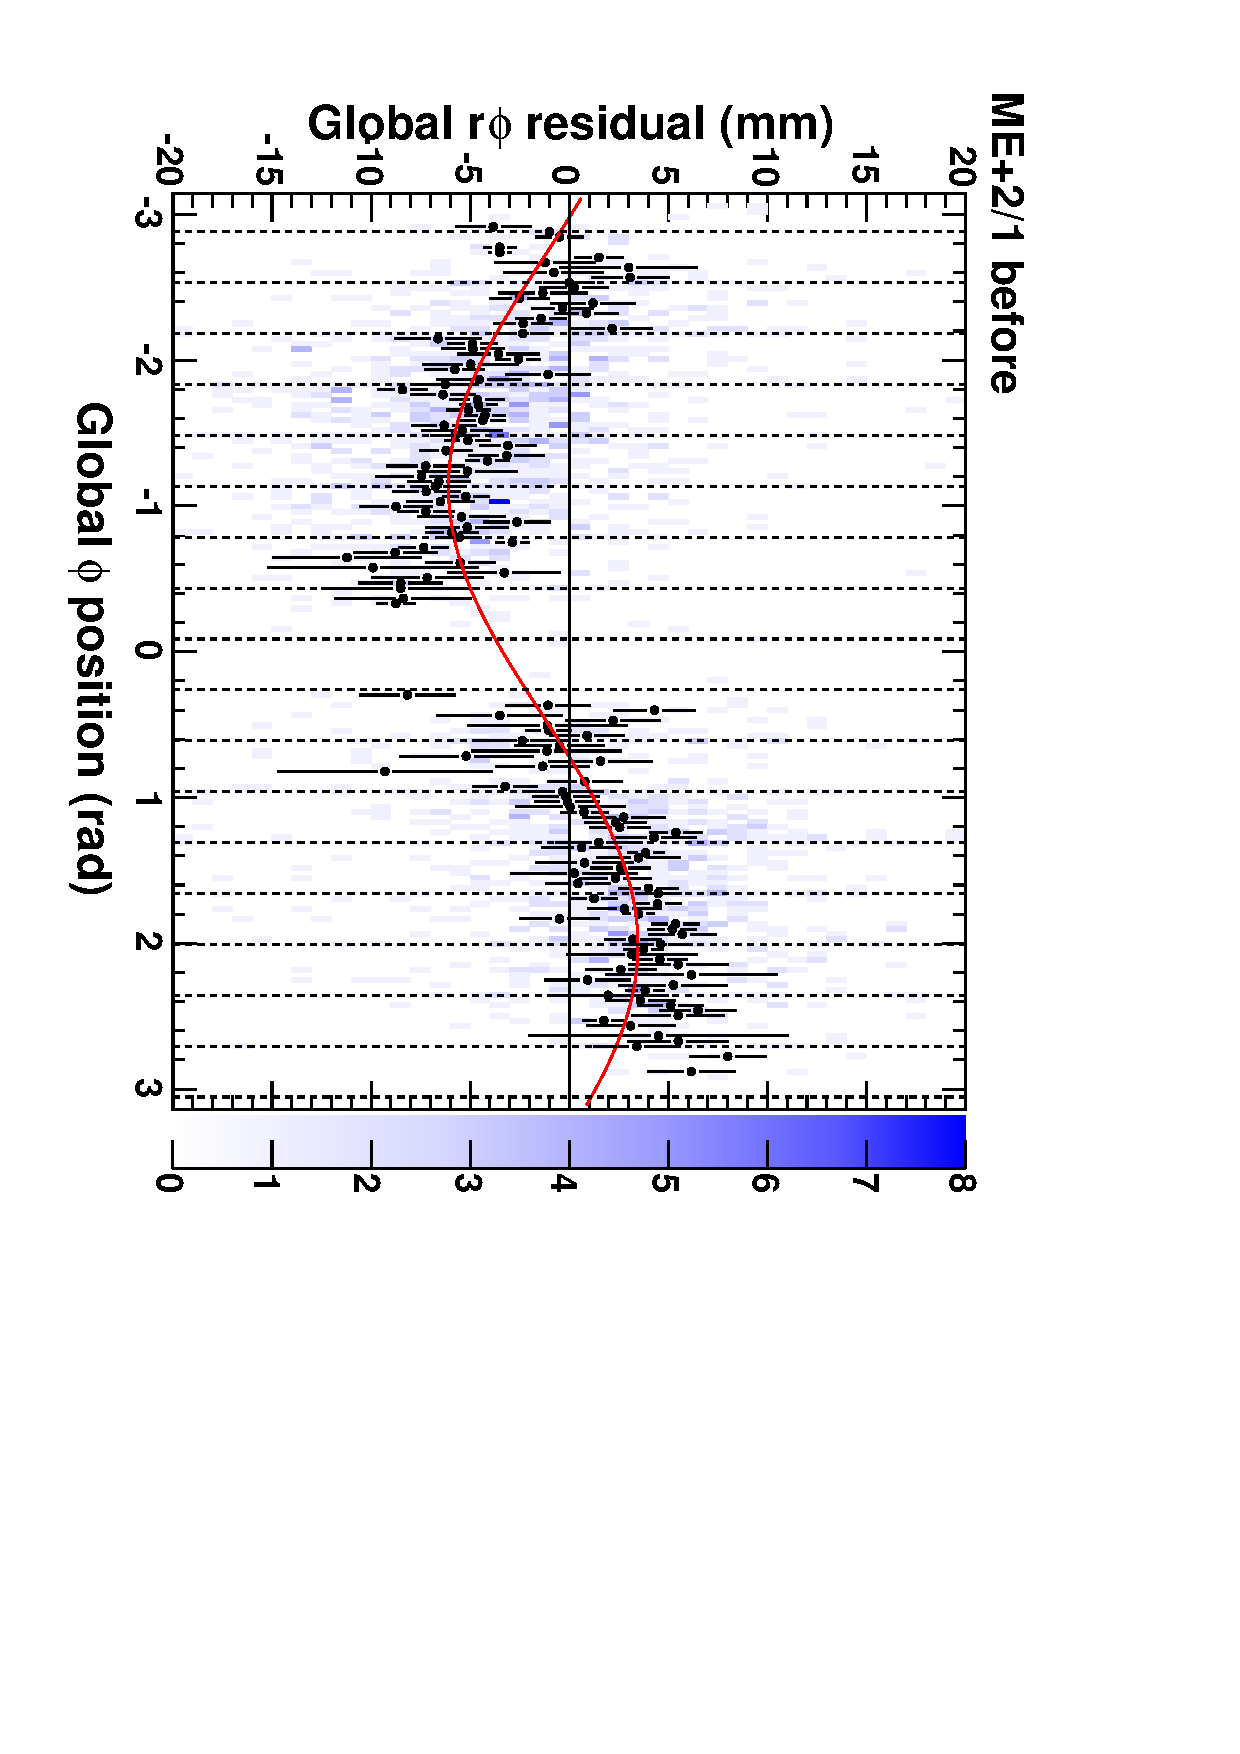
\includegraphics[height=0.5\linewidth, angle=90]{inneralignment_before.pdf}
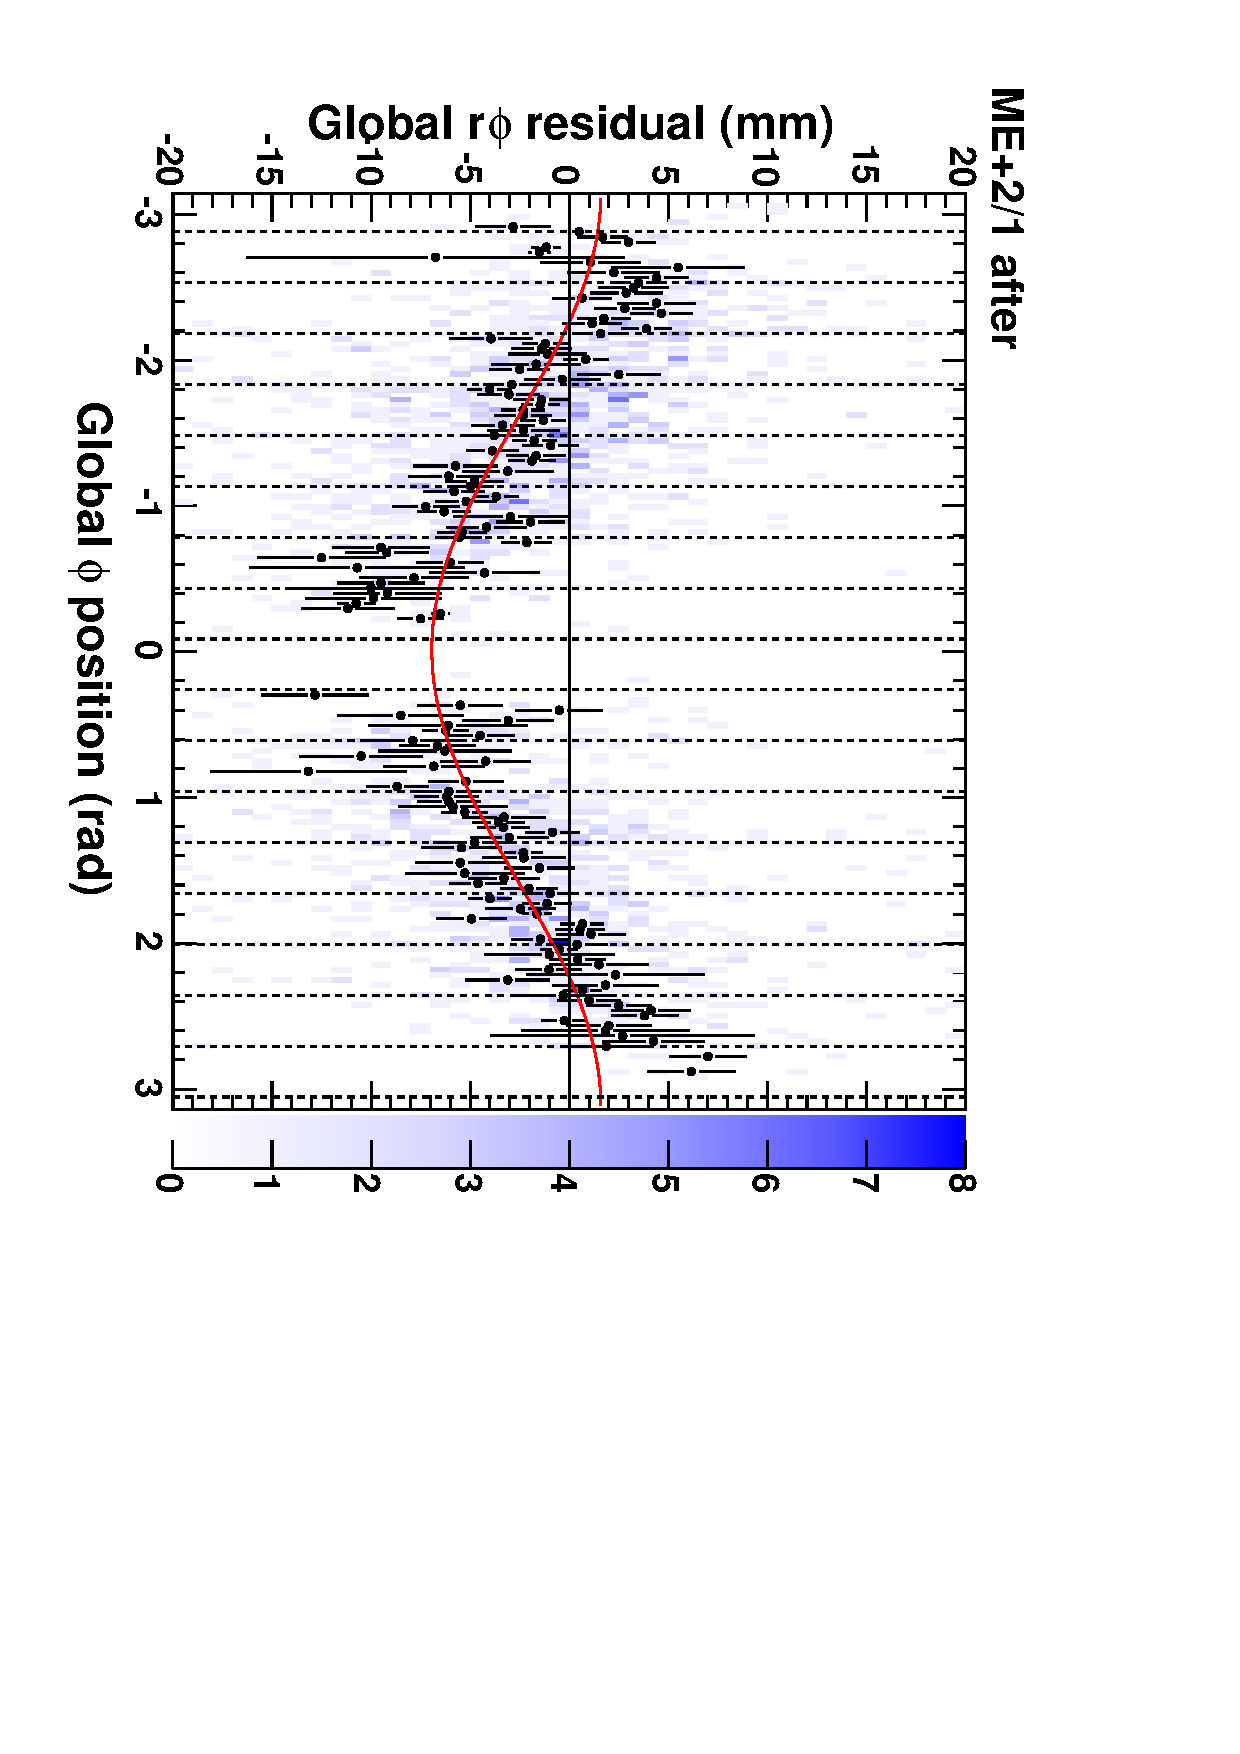
\includegraphics[height=0.5\linewidth, angle=90]{inneralignment_after.pdf}

\begin{itemize}
\item What are the prospects of getting DCOPS input?  ($\delta_z$ and $\delta_{\phi_x}$)
\end{itemize}
\end{frame}

\begin{frame}
\frametitle{Endcap residuals bug hunt}
\renewcommand{\arraystretch}{1.8}
\mbox{\hspace{-0.5 cm}\begin{tabular}{c p{0.6\linewidth} p{0.35\linewidth}}
$\surd$ & check all ideal chamber center positions (database and DDD) & no 22X $\to$ 3XY changes \\
$\surd$ & check all strip positions relative to chamber centers (Tim Cox) & no 22X $\to$ 3XY changes \\
$\surd$ & ask all reconstruction experts about other changes & no leads \\
$\surd$ & create a CSC overlaps skim of CRAFT-2009 & done, waiting for me to analyze \\
& dump all aspects of overlap discrepancies, determine at what level the error occurs & \\
& does it affect reconstruction in general? & \\
& re-reconstruct CRAFT-2008 data in 3XY: might this be a read-out issue in 2009, rather than reconstruction in 3XY? (hopefully not!) & \\
\end{tabular}}
\end{frame}

\begin{frame}
\frametitle{TID/TEC study (1/5)}
\begin{itemize}
\item Can we now use the tracker TID/TEC in muon barrel alignments?
\item All of the following plots: difference in aligned positions using
\begin{enumerate}[(\alph{enumi})]
\item tracks with zero TID/TEC hits (previous alignments)
\item tracks with one or more TID/TEC hits \mbox{(statistically independent)\hspace{-1 cm}}
\end{enumerate}
\item Dashed reference is same in infinite-statistics ideal-tracker \mbox{cosmics MC\hspace{-1 cm}}
\end{itemize}

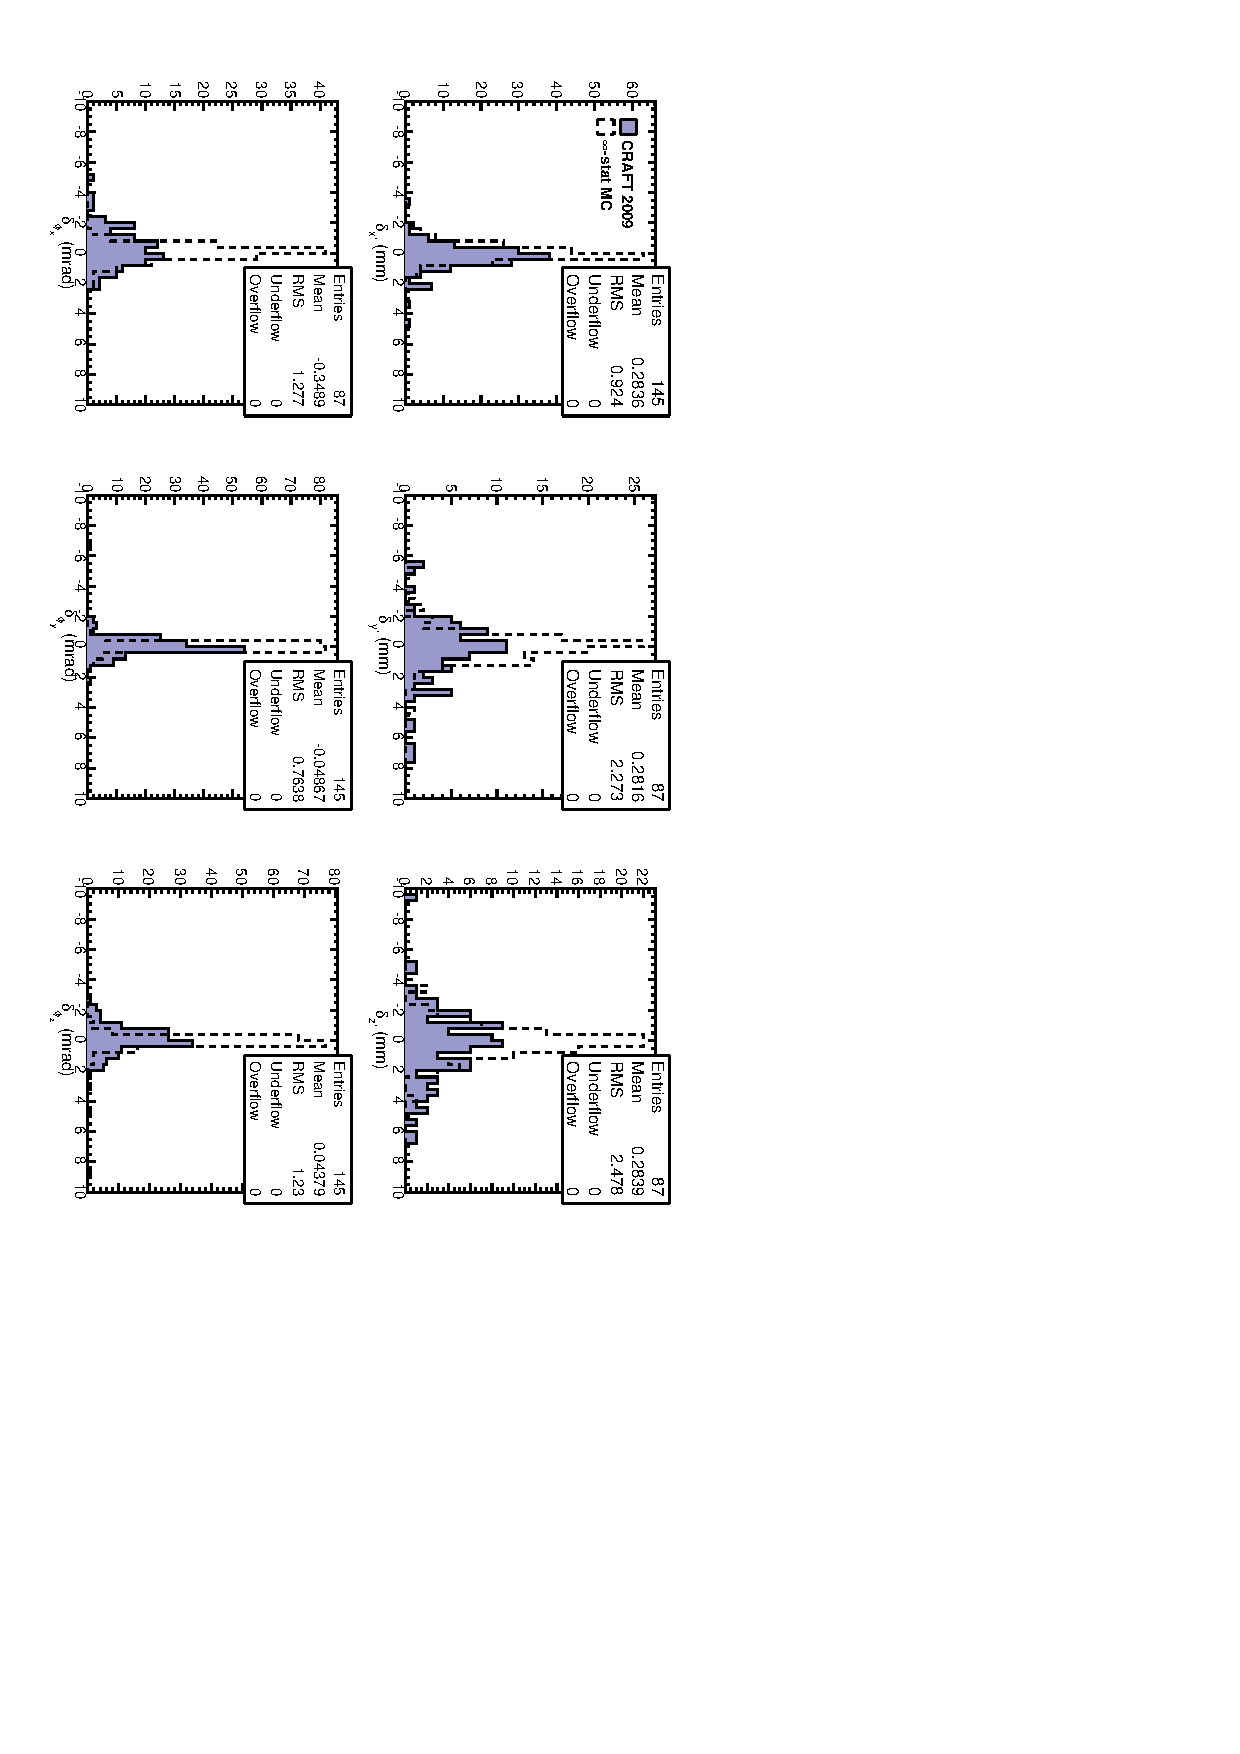
\includegraphics[height=\linewidth, angle=90]{tecdiff.pdf}
\end{frame}

\begin{frame}
\frametitle{TID/TEC study (2/5)}
\begin{itemize}
\item Data: more spread than MC, with 0.28~mm bias (tracker TID/TEC vs.\ TIB/TOB misalignment?)
\item More spread in wheels $\pm$2, but that is due to lower statistics
\end{itemize}

\begin{columns}
\column{0.5\linewidth}
\begin{center}
wheels $-$1, 0, $+$1
\end{center}
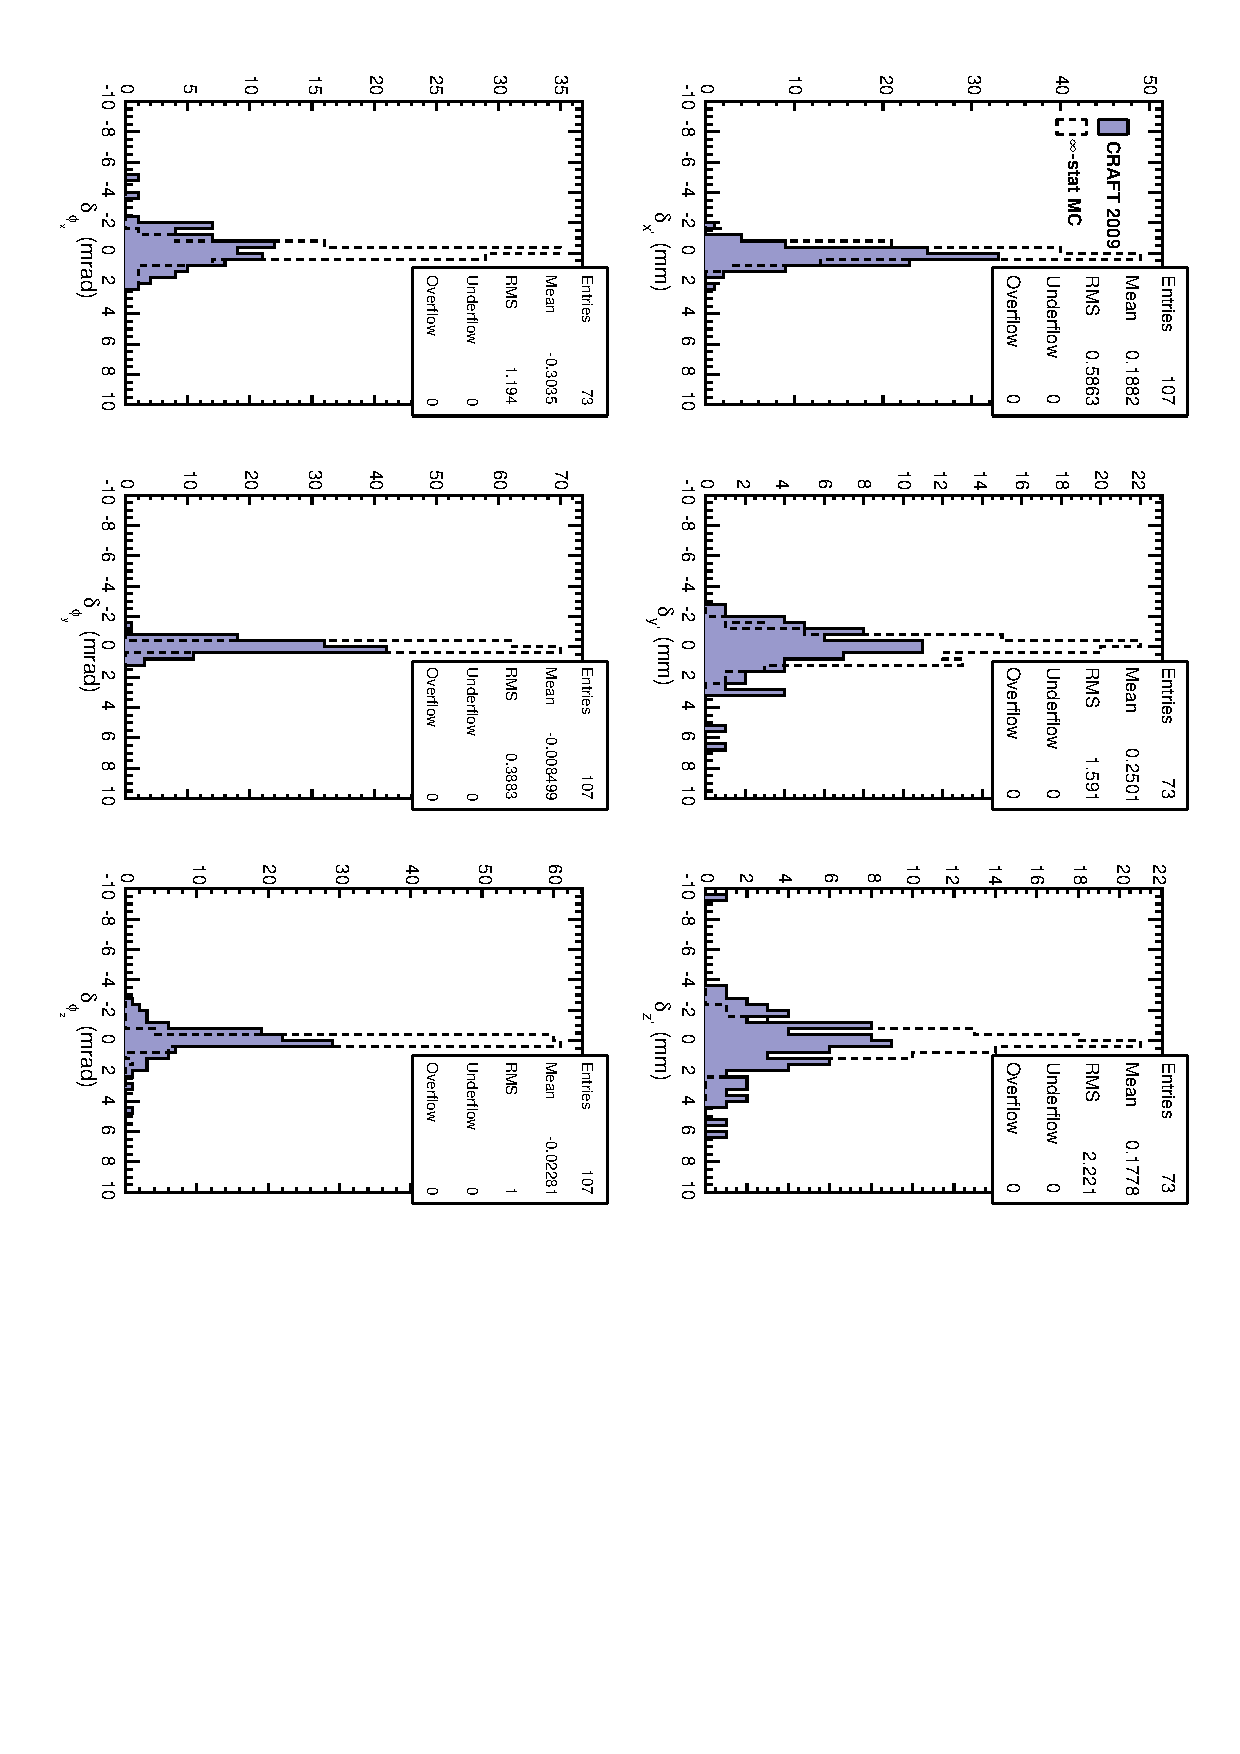
\includegraphics[height=\linewidth, angle=90]{tecdiff_central.pdf}

\column{0.5\linewidth}
\begin{center}
wheels $-$2, $+$2
\end{center}
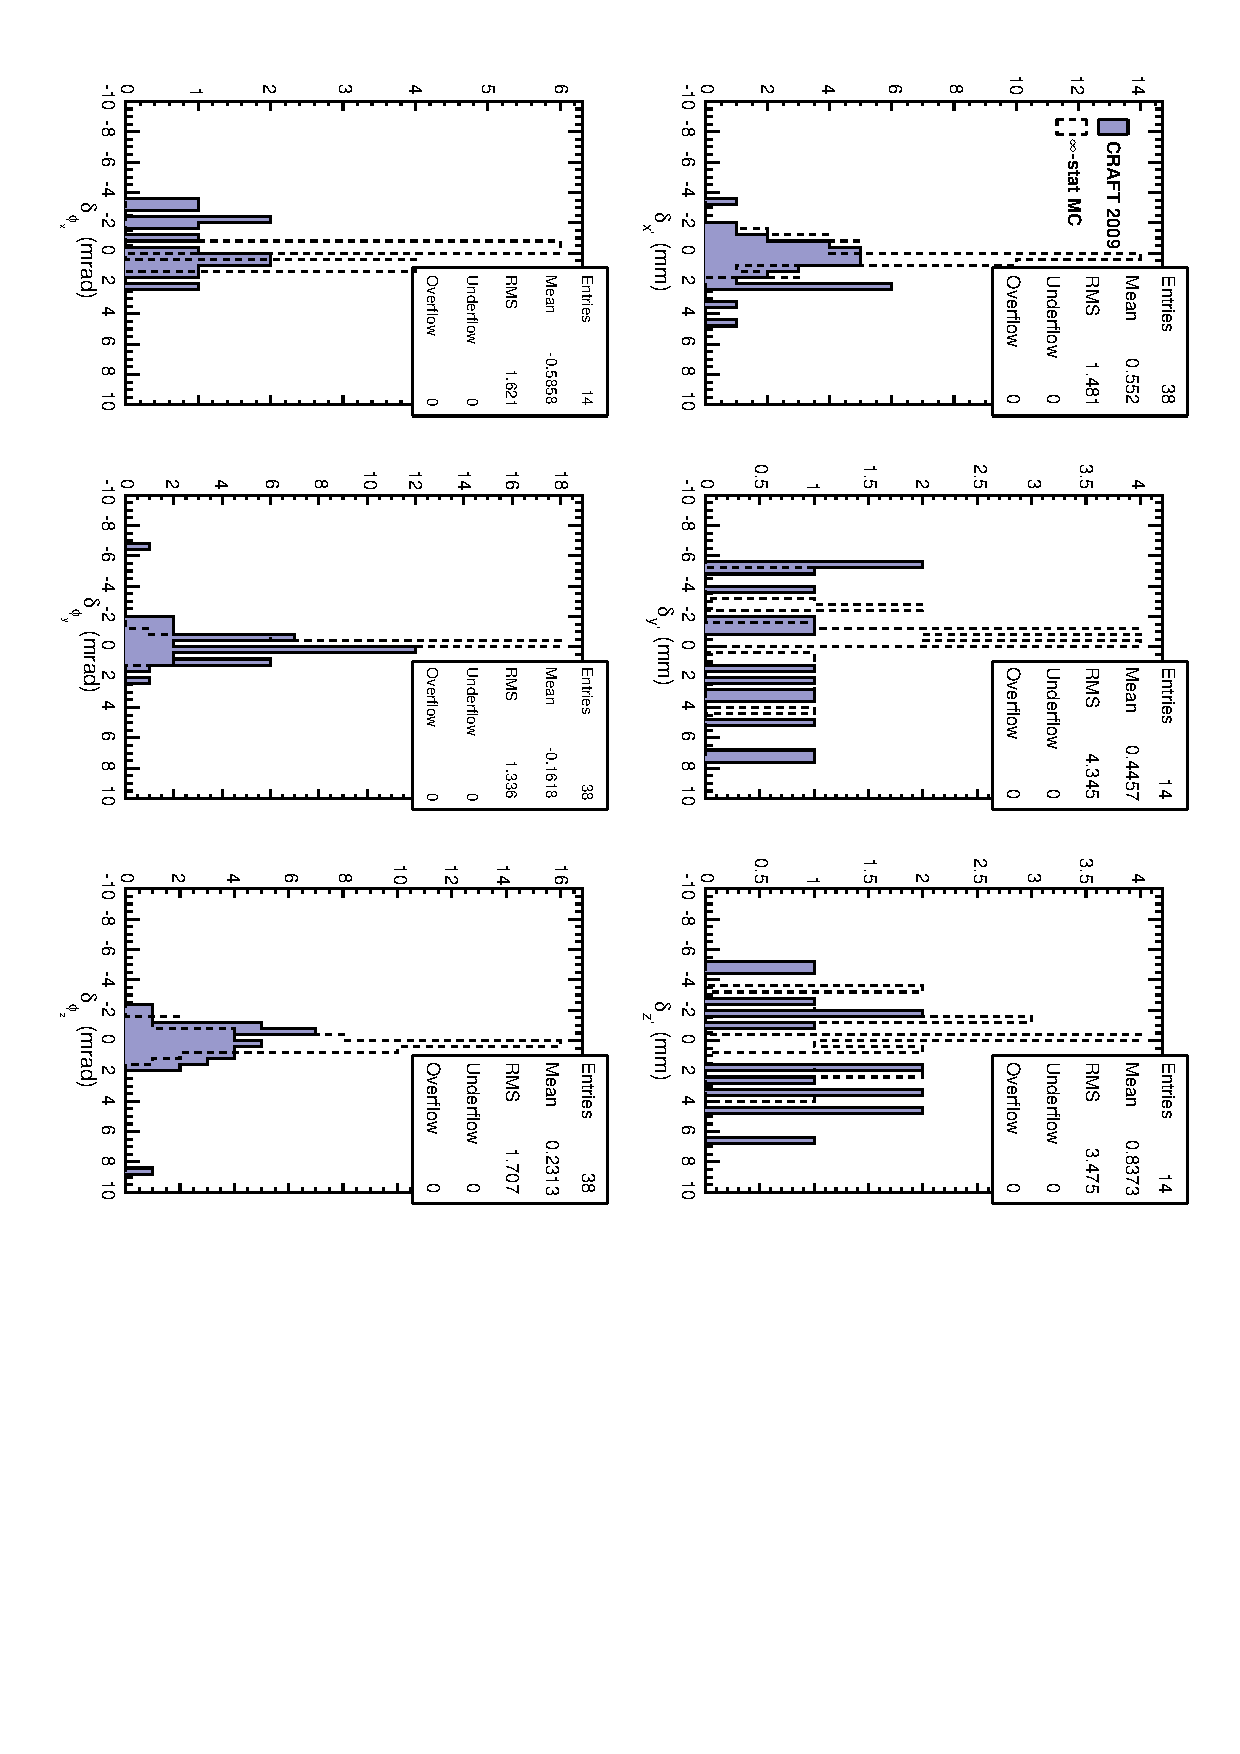
\includegraphics[height=\linewidth, angle=90]{tecdiff_outer.pdf}
\end{columns}
\end{frame}

\begin{frame}
\frametitle{TID/TEC study (3/5)}
\begin{itemize}
\item To study statistics, plot position difference ($\delta_x$) over
  statistical uncertainty ($\sigma_x$)
\item Blue reference is a unit Gaussian (purely statistical deviations)
\item Statistically significant excess at high $\delta_x$
\end{itemize}

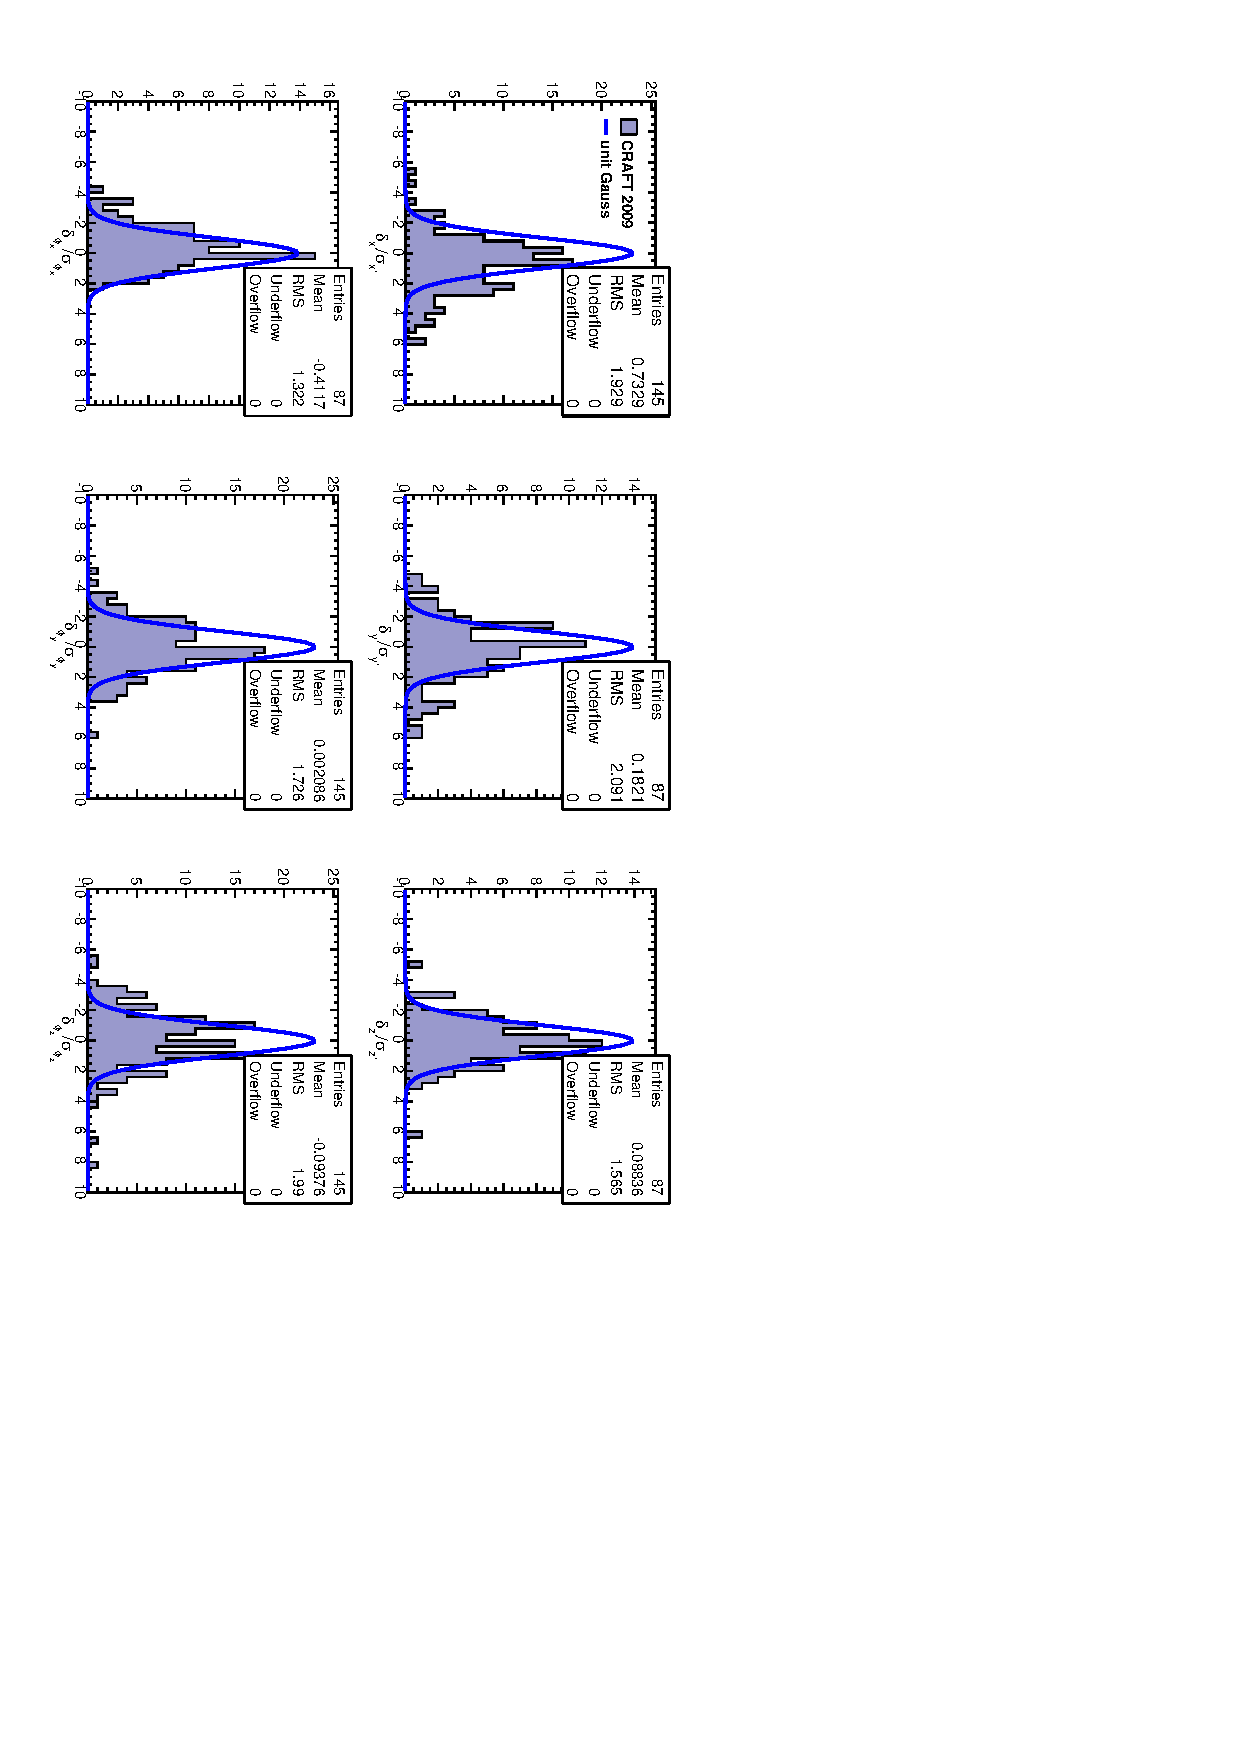
\includegraphics[height=\linewidth, angle=90]{tecnorm.pdf}
\end{frame}

\begin{frame}
\frametitle{TID/TEC study (4/5)}
\begin{itemize}
\item It's no more significant in wheels $\pm$2 than central wheels
\item That's why we can conclude that the larger spread on p.~6 is statistical
\end{itemize}

\begin{columns}
\column{0.5\linewidth}
\begin{center}
wheels $-$1, 0, $+$1
\end{center}
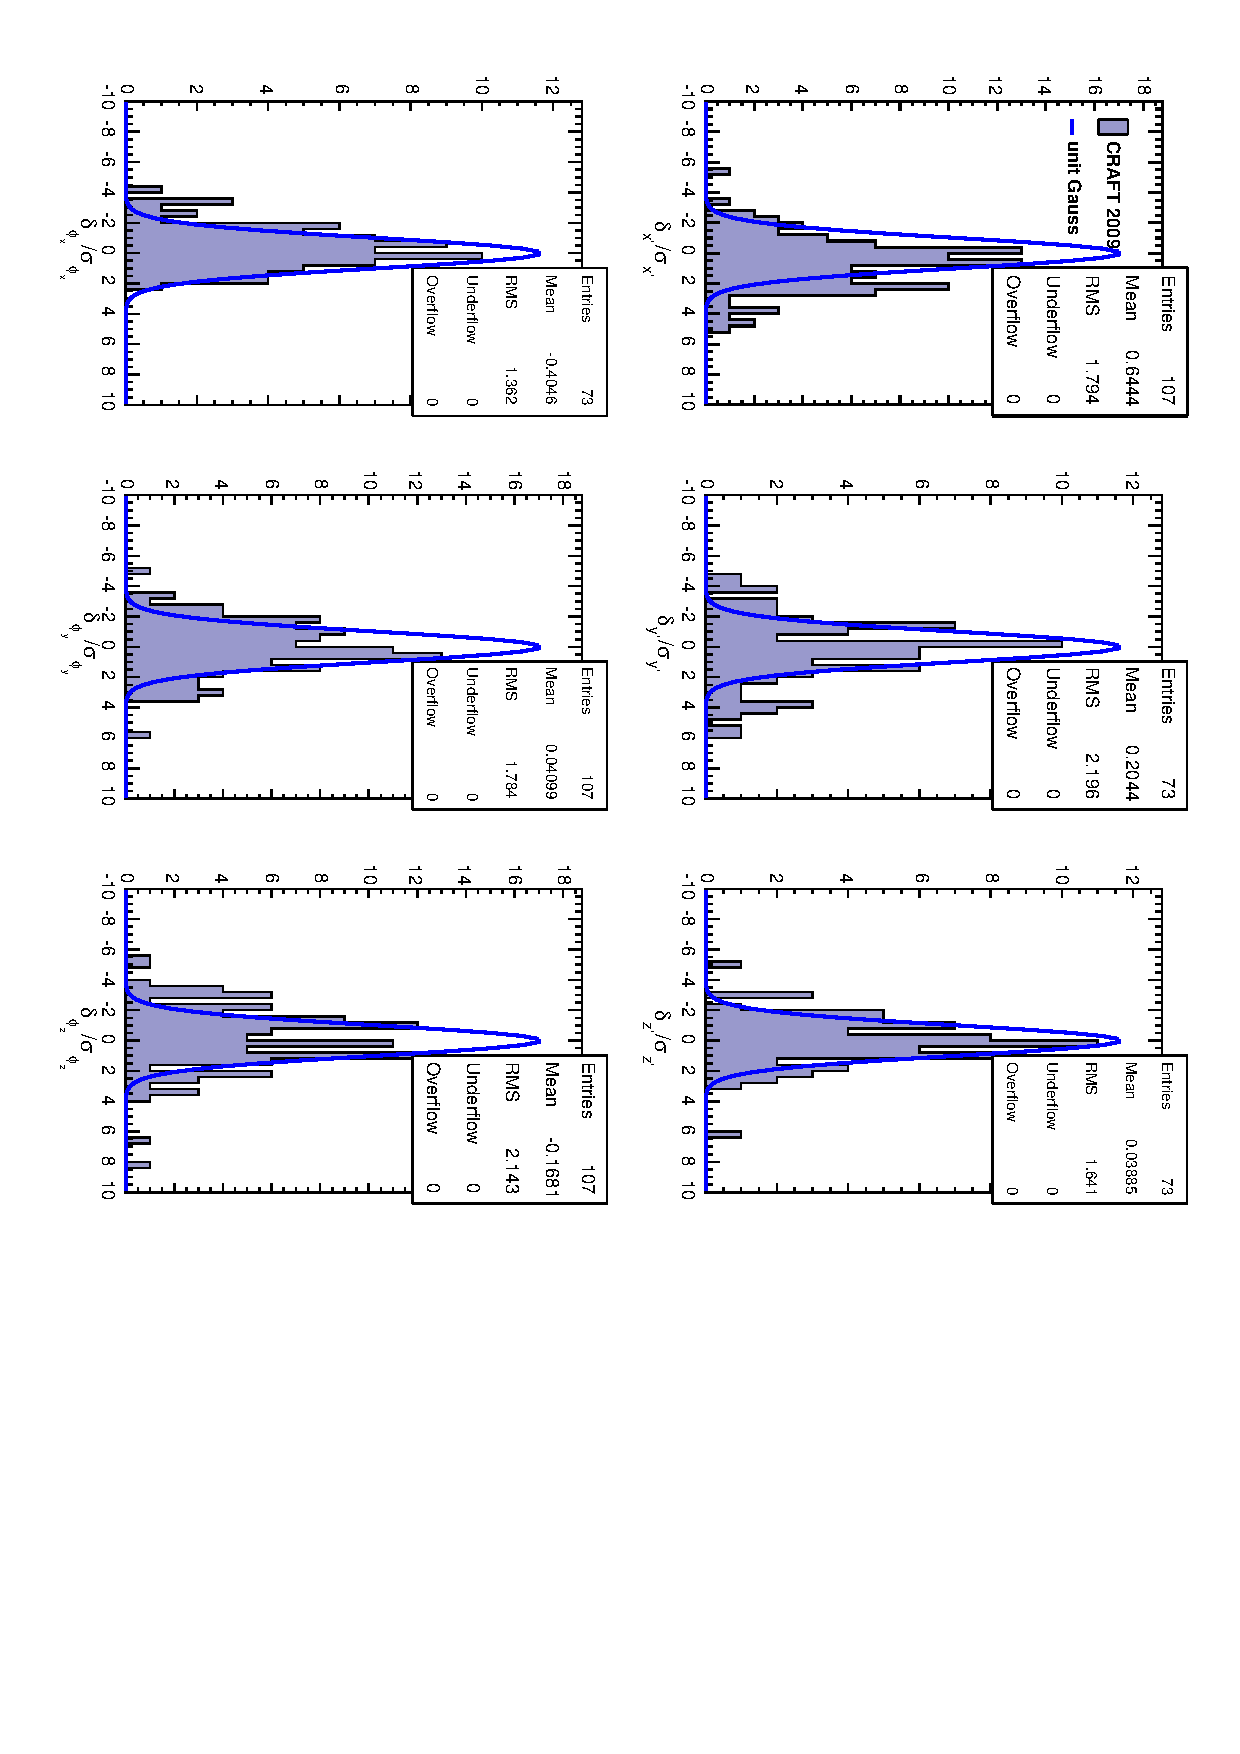
\includegraphics[height=\linewidth, angle=90]{tecnorm_central.pdf}

\column{0.5\linewidth}
\begin{center}
wheels $-$2, $+$2
\end{center}
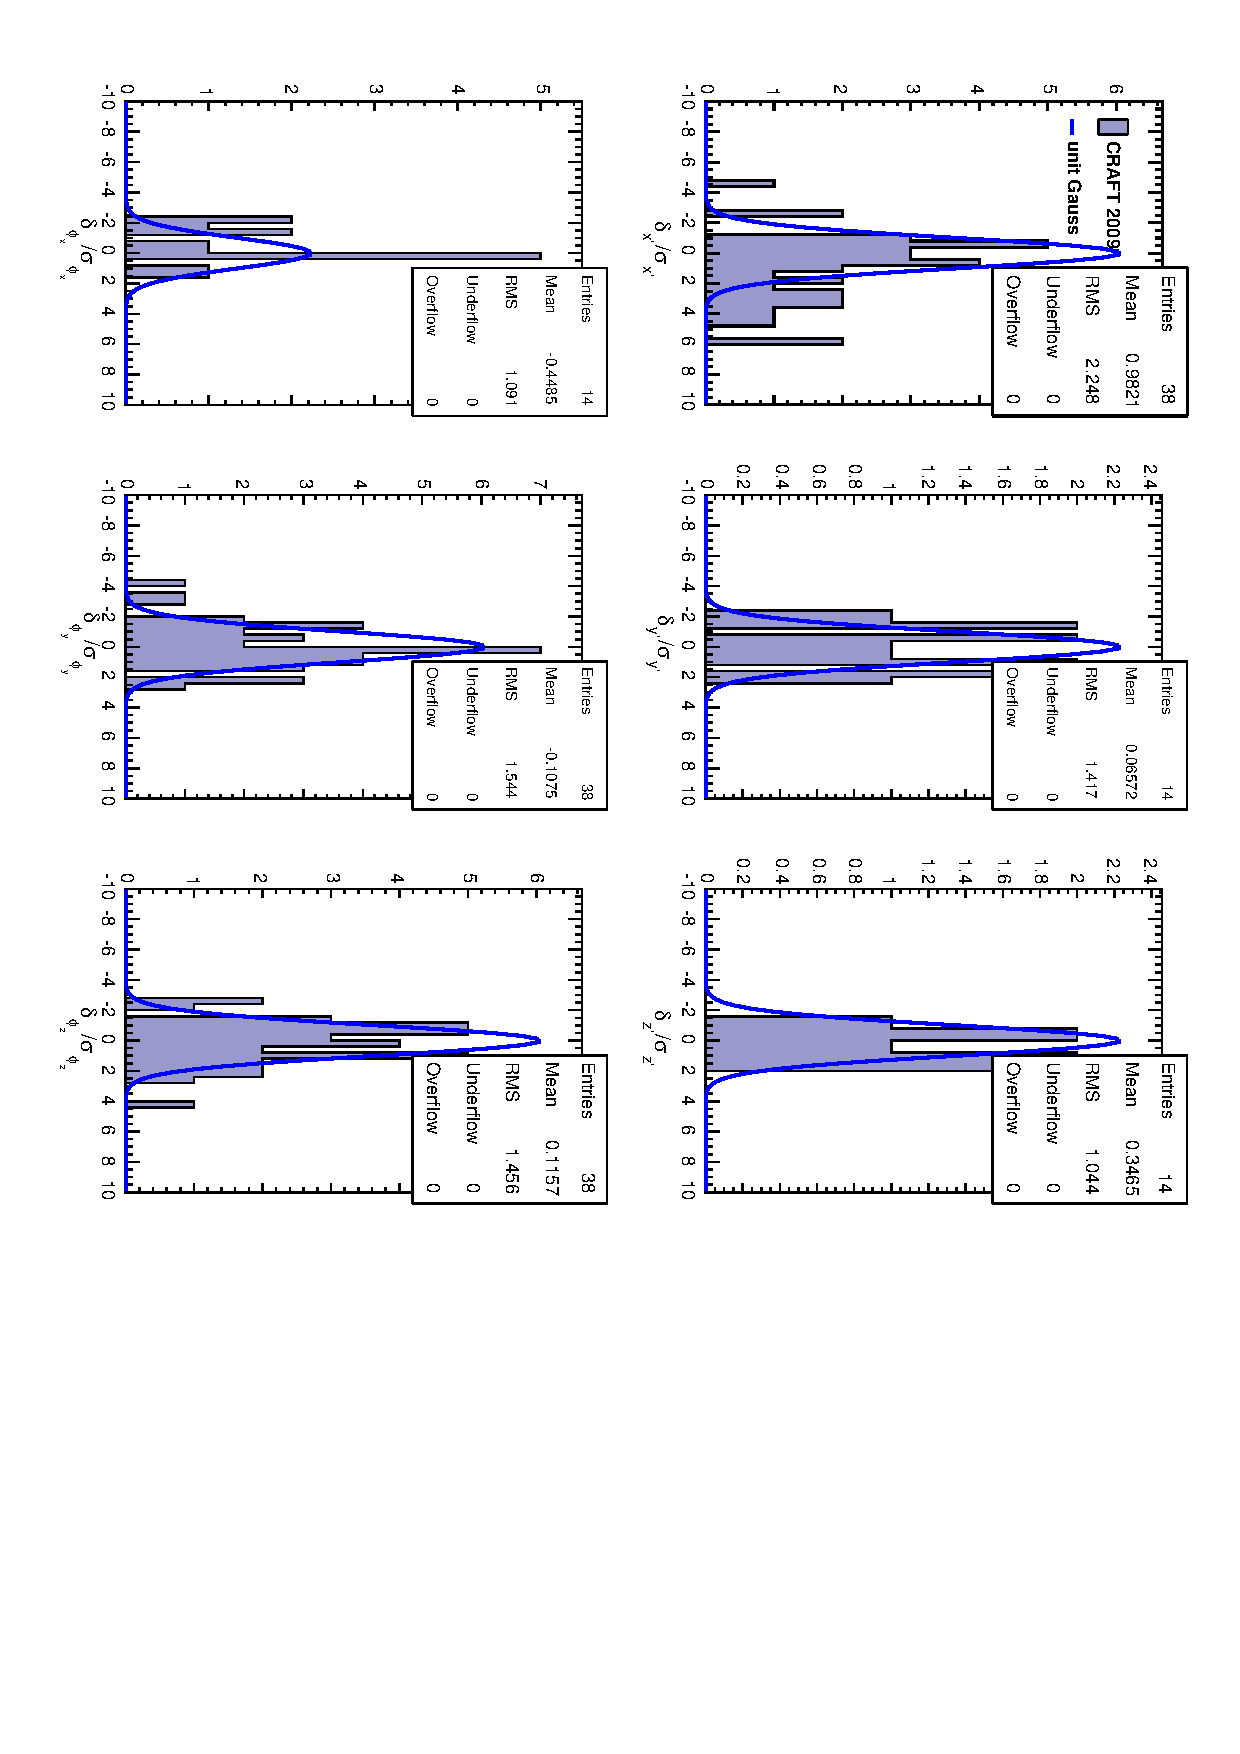
\includegraphics[height=\linewidth, angle=90]{tecnorm_outer.pdf}
\end{columns}
\end{frame}

\begin{frame}
\frametitle{TID/TEC study (5/5)}
\begin{itemize}
\item No global patterns in $\delta_\phi = \delta_x/R$ vs.\ $\phi$
\item Mean $\delta_\phi$ is 0.04~mrad
\item Can be more precisely studied by plotting muon residuals as a
  function of their origin in the tracker (old ``tracker X-ray plots'')
\end{itemize}

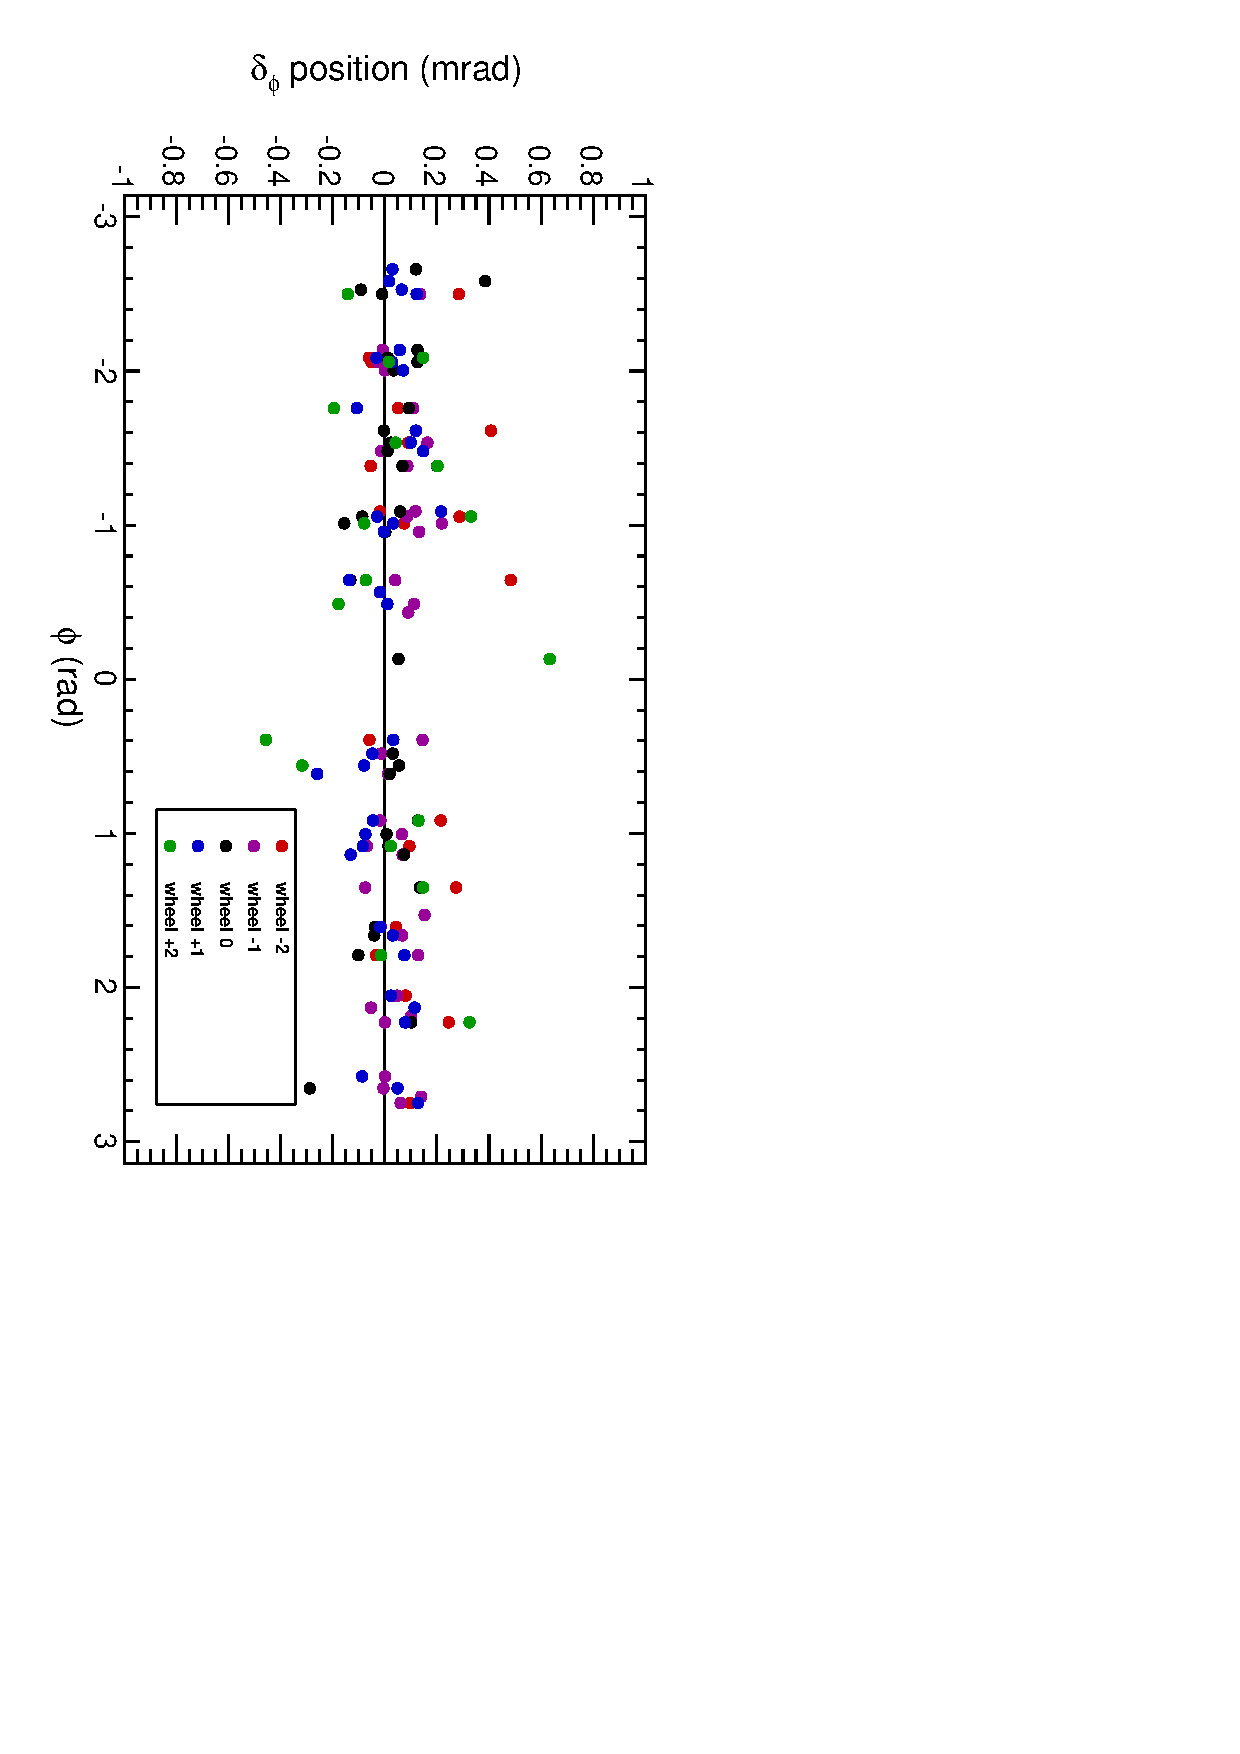
\includegraphics[height=\linewidth, angle=90]{tecphi.pdf}
\end{frame}

\begin{frame}
\frametitle{Summary}
\begin{itemize}\setlength{\itemsep}{0.25 cm}
\item Ring-1 chambers, unaffected by bug, allow us to align endcap disks
\begin{itemize}
\item corrected sign and resubmitted
\item any news on DCOPS-based input, to make a \mbox{merged alignment?\hspace{-1 cm}}
\end{itemize}

\item Bug hunt continues: today I'll be looking at the overlap hits
  (and their strip numbers, position in strip, etc.)

\item Statistically sensitive to a small bias from the TID/TEC
\begin{itemize}
\item bias of 0.04~mrad rotation (0.28~mm $\delta_x$ translations)
  between tracks with no TID/TEC hits and tracks with at least one TID/TEC hit
\item spread in chamber positions (0.9~mm) dominated by statistical
  errors, especially in wheels~$\pm$2
\item I would advocate using all tracker tracks in the next alignment
\end{itemize}

\item The next track-based alignment will inherit $\delta_{\phi_x}$
  angles from a prior measurement.  Will that prior measurement be
  photogrammetry, and is there an SQLite input geometry available?
\end{itemize}

\label{numpages}
\end{frame}

\end{document}
